% File: src/chapter_5_implementation.tex
% Project: Monitoring and Reporting Tool for Cloned Vulnerabilities across Open-Source Projects
% Author: Matus Remen (xremen01@stud.fit.vutbr.cz)
% Description: Chapter 5 - Implementation

\chapter{Implementation}
\label{chapter:implementation}
  This Chapter outlines the implementation of the tool designed to scan and detect cloned vulnerabilities in open-source projects.
  The tool leverages a~modern technology stack, consisting of Python~3\footnote{\href{https://www.python.org/downloads/}
  {https://www.python.org/downloads/}} for the backend and the API, Redis and PostgreSQL
  for databases and ReactJS for the web interface. Additionally, the entire application is containerized using
  Docker Compose\footnote{\href{https://docs.docker.com/compose/}{https://docs.docker.com/compose/}},
  which offers organized management of multiple services displayed in Figure~\ref{cg-services}.
  By leveraging the mentioned technologies, the tool provides an efficient and user-friendly solution for identifying
  cloned vulnerabilities in open-source software, thus contributing to secure software development practices.

  \begin{figure}[h]
    \centering
    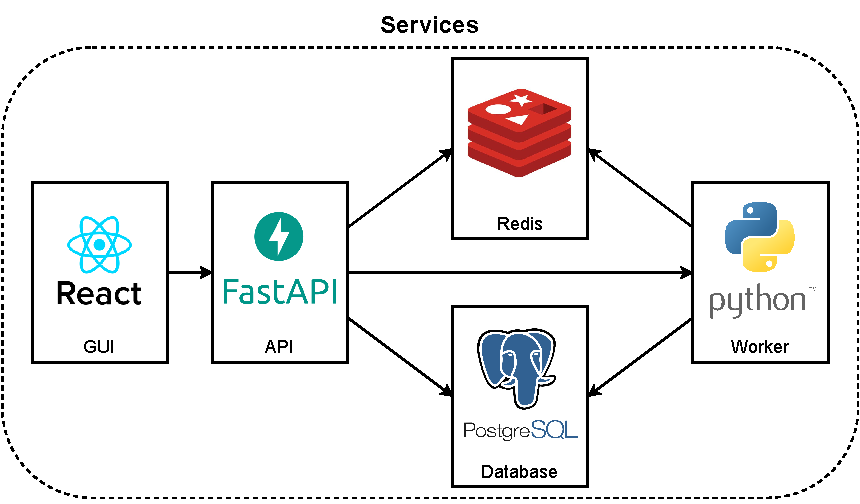
\includegraphics[width=0.7\textwidth]{obrazky-figures/cg_services.drawio.pdf}
    \caption{An overview of the services constructing the tool and their mutual dependencies.}
    \label{cg-services}
  \end{figure}

  For the development of the major part of the tool, Python~3 was chosen, a~versatile and widely used programming language known for its
  readability and ease of use. As the tool uses various technologies, the main benefit of this choice is versatility,
  which assures compatibility between particular parts of the tool and communication with various external APIs.
  In the transition from API to the backend and its detection methods, the choice of Python as the development language
  plays a~significant role in integrating key architectural elements, such as the Redis\footnote{\href{https://redis.io/docs/about/}{https://redis.io/docs/about/}} and
  PostgreSQL\footnote{\href{https://www.postgresql.org}{https://www.postgresql.org}} database. Although, it could suffer
  from execution speed in the case of detection methods in comparison to the programming language C++~\cite{hackrPythonVSCPP}.

  \section{Storage}
  Overall, there are three types of storage used by the tool: the database, the local storage and in-memory storage -- Redis.
  This Section will describe the implementation and usage of each type.

  \subsection*{Database}
  \label{impl:database}
  The internal database is the first type of utilized storage, which is used for storing long-term data, containing
  essential configurations for the tool and results of the detection method. For the implementation of the schema designed
  in Section~\ref{design:database} an open-source object-relational database management system PostgreSQL was selected
  for its great ability to scale. PostgreSQL provides a~docker image, which eases the integration to the tool
  thanks to the usage of containerization via Docker Compose.

  The connection to the database is established using a~Python library \texttt{psycopg2}\footnote{\href{https://www.psycopg.org/docs/}
  {https://www.psycopg.org/docs/}} an efficient, low-level PostgreSQL database adapter performing
  basic database operations. Additionally, an Object Relational Mapper (ORM) library
  \texttt{SQLAlchemy}\footnote{\href{https://www.sqlalchemy.org}{https://www.sqlalchemy.org}}
  is used to simplify access and operations with database objects.
  It provides a~high-level, object-oriented interface that abstracts the underlying database system and allows it to work
  during the development with Python classes instead of raw SQL queries.

  To access the features of the \texttt{SQLAlchemy}, the schema of tables in the database is implemented in Python classes which
  inherit from \texttt{DeclarativeBase} class provided by the library. That defines at once both, the Python object model
  and database metadata that describe tables in the database. According to the designed database schema, the tool implements
  classes \texttt{Bug}, \texttt{Project} and \texttt{Detection} this way.

  To improve readability and developer experience, the tool implements an interface abstracting all operations with the tables
  in the database. The interface is available in a~CRUD module, which implements all used variants of queries to Create, Read,
  Update and Delete records in the database in one place.

  \subsection*{Local Storage}
  \label{impl:local-storage}
  The second type of storage used by the tool is its own local storage on the hosting file system. It is used for storing clones of registered repositories
  and logs from the detection method. During the execution of the detection method, all operations and commands with the analysed
  projects are performed on the clones stored here. By fetching the log files stored here, the API provides data for the page
  displaying detection results in the web interface.

  \subsection*{Redis}
  \label{impl:redis}
  Redis is an open-source, in-memory data structure store used by this tool as a~cache storing a~queue of scheduled
  requests for execution of detection method. As in-memory storage, Redis provides very fast read and write actions,
  and it supports a~wide variety of data structures. Additionally, it is distributed also as a~docker image, which allows
  easy integration of the service using Docker Compose. The connection
  and operations with Redis are assured by a~Python library \texttt{redis}\footnote{\href{https://redis.io/docs/clients/python/}
  {https://redis.io/docs/clients/python/}}.

  To initialize and manage the aforementioned queue in Redis a~Python library \texttt{rq}\footnote{
  \href{https://github.com/rq/rq}{https://github.com/rq/rq}} is used, which stands for Redis Queue. The purpose of this library
  is to schedule jobs for processing in the background and extend the options of the tool in terms of scalability. In the
  implementation of the tool, the jobs are queued by an API and processed by the worker service.

  \section{Detection Mechanism and its Components}
  The detection mechanism is the core component of the tool developed in this project. It is implemented using the programming
  language Python~3 and an object-oriented approach. The mechanism requires on the input an identification of a~bug and the name of the project
  where it was discovered. Accordingly, at the beginning of the workflow, the mechanism finds a~fixing commit of the provided vulnerability,
  parses important details and creates an object representing the bug.

  \begin{figure}[h]
    \centering
    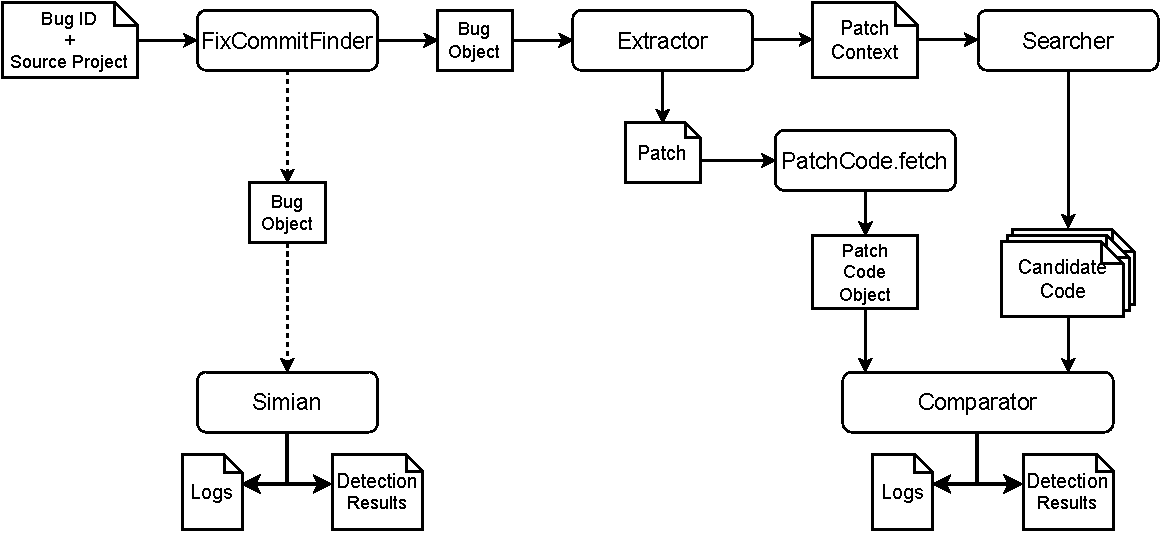
\includegraphics[width=1\textwidth]{obrazky-figures/cg_impl_detection.drawio.pdf}
    \caption{Workflow of the default detection method, with an optional alternative method using tool Simian. Both
             methods process the same Bug Object created after processing the detection request
             specifying the Bug ID and the project where it originated.}
    \label{cg-impl-detection}  % TODO add step with initialization of projects
  \end{figure}

  At this point, the mechanism offers two methods for detecting the propagation of the bug among the forks of the source project.
  The first method utilizes a~tool Simian, which has great performance but is able to detect only clones of the first type.
  The second, default method is inspired by the approach of the tool BlockScope, which is capable of detecting clones of Type~I,
  Type~II and Type~III.

  The complete workflow of the mechanism and its components is displayed in Figure~\ref{cg-impl-detection}. The components
  of the workflow and its implementation will be described in the following subsections.

  \subsection*{Component \texttt{FixCommitFinder}}
  Upon execution of the detection mechanism, the component \texttt{FixCommitFinder} is the first functional part of the workflow.
  It is developed as a~class implementing methods for finding bug-fixing commits for both, the targeted detection
  and discovery scan.

  \begin{figure}[h]
    \centering
    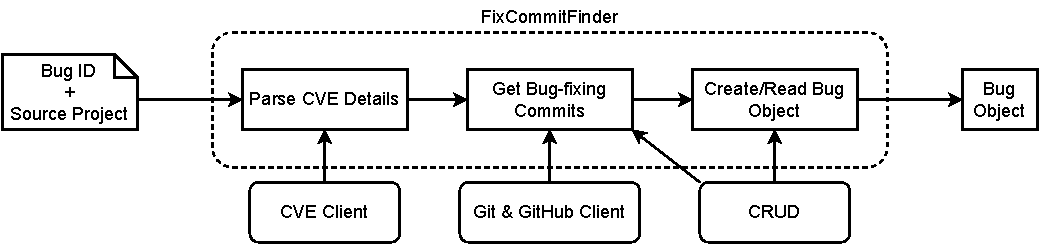
\includegraphics[width=0.9\textwidth]{obrazky-figures/cg_impl_fixcommitfinder.drawio.pdf}
    \caption{Workflow of the component \texttt{FixCommitFinder} in targeted detection. In the case of CVE ID, the component
             parses and uses its details to find bug-fixing commit in the source repository. The fix commits can be supplied
             from the internal database using the CRUD interface.}
    \label{cg-impl-fixcommitfinder}
  \end{figure}

  The process of the component \texttt{FixCommitFinder} in targeted detection is described in Figure~\ref{cg-impl-fixcommitfinder}.
  If the given bug ID is available in the internal database, the final bug object is fetched from there using the CRUD interface
  and returned. Otherwise, if a~CVE is provided, a~class \texttt{CVEClient} is used for parsing its details. The class utilizes a~Python~3 library
  \texttt{requests}\footnote{\href{https://docs.python-requests.org/en/latest/index.html}
  {https://docs.python-requests.org/en/latest/index.html}} for retrieving the data from National Vulnerability Database API using
  HTTP requests. Subsequently, the references to a~fixing commit, pull request or release notes in details about the vulnerability
  are parsed. If the references are not available or recognized, the component additionally extracts keywords from the description
  of the vulnerability using a~library \texttt{nltk}\footnote{\href{https://www.nltk.org}{https://www.nltk.org}}. All extracted details
  are then used for finding the bug-fixing commits using commands of tool \texttt{git}\footnote{\href{https://git-scm.com}
  {https://git-scm.com}} and GitHub API\footnote{\href{https://docs.github.com/en/rest}{https://docs.github.com/en/rest}} available
  in a~class \texttt{Git}. In the end, if the bug ID was not available in the internal database before, the component creates a~new
  object \texttt{Bug}, stores it and returns. A~visualisation of the returned object is available in Figure~\ref{cg-impl-bug-object}.

  \begin{figure}[h]
    \centering
    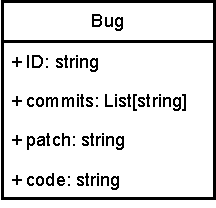
\includegraphics[width=0.25\textwidth]{obrazky-figures/cg_impl_bug_object.drawio.pdf}
    \caption{Overview of the object \texttt{Bug} and its utilized attributes.}
    \label{cg-impl-bug-object}
  \end{figure}

  For the discovery scan, a~different method of the component is used and its workflow is displayed
  in Figure~\ref{cg-impl-fixcommitfinder-scan}. This method requires the on input only the object of the repository
  which will be scanned for new bug-fixing commits for the past couple of days. In the end, this process returns a~list of suspicious
  commits which were detected by a~keywords representing a~software weaknesses or a~patch action in commit messages.

  \begin{figure}[h]
    \centering
    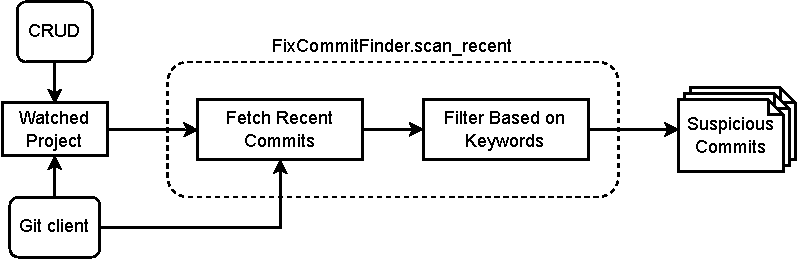
\includegraphics[width=0.9\textwidth]{obrazky-figures/cg_impl_fixcommitfinder_scan.drawio.pdf}
    \caption{Overview of a workflow of the component \texttt{FixCommitFinder} using method for discovery scan.}
    \label{cg-impl-fixcommitfinder-scan}
  \end{figure}

  \subsection*{Component \texttt{BlockScope}}
  The default method of the detection mechanism is based on the approach proposed in the paper about a~tool BlockScope,
  which was described in Section~\ref{section:blockscope}. The implementation of particular components involved in this method
  slightly diverged as it is visible on the right side of Figure~\ref{cg-impl-detection}.

  The component \texttt{Fetcher} from the original design is omitted and its functionality was inherited by the component
  \texttt{Searcher} and a~method of the object \texttt{PatchCode}. It was implemented this way to encapsulate every attribute
  and action related to the patch into one object as during extraction of the patch code is done an additional analysis of structure,
  thus type of the patch is. The component \texttt{Searcher} in this design implements both the context-based search process
  for localization of candidate code in the target repository and extraction of the candidate code.

  Each part of the method produces logs, which can be observed on the web. In the end, if the final result of the detection
  is that the analysed project did not apply the patch, the result is additionally archived in the internal database.

  \subsection*{Component \texttt{Simian}}
  Simian\footnote{\href{https://www.harukizaemon.com/simian}{https://www.harukizaemon.com/simian}} is a~tool for detecting
  code duplicates. It is integrated into the detection mechanism as an alternative method for analysing vulnerable code duplication
  between the source project and its forks. Simian is implemented in the programming language Java, so for its execution was implemented an interface
  as a~separate component, which was named after the tool. The interface also implements a~parser for its output.
  An example output of the tool and parsed information is displayed in Figure~\ref{cg-impl-simian-output}.

  \begin{figure}[h]
    \centering
    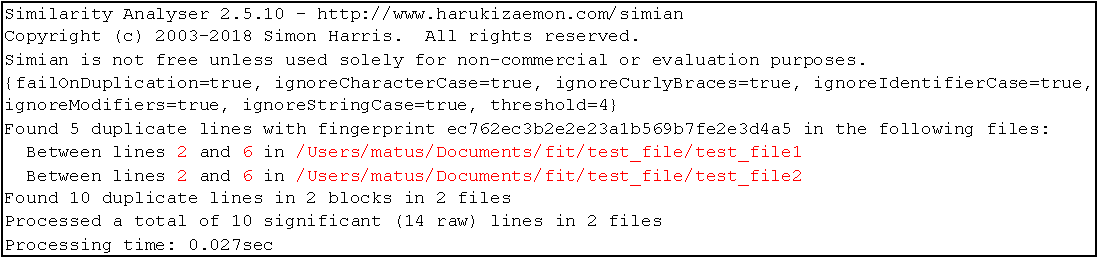
\includegraphics[width=0.9\textwidth]{obrazky-figures/cg_impl_simian_output.drawio.pdf}
    \caption{Output from Simian with highlighted information that is parsed in the detection mechanism.}
    \label{cg-impl-simian-output}
  \end{figure}

  \section{Application Programming Interface}
  The application programming interface (API) is an important part of the tool as it controls communication between the GUI
  and the core of the application. For the implementation of the REST API was chosen Python web framework FastAPI\footnote{
  \href{https://fastapi.tiangolo.com}{https://fastapi.tiangolo.com}}. It achieves great performance, supports
  asynchronous programming and automatically generates API documentation. The implementation of API endpoints
  will be described in the rest of the section.

  \subsection*{API Endpoints}
  \label{impl:api}
  The implemented API contains overall 9 endpoints which deliver messages between the frontend and backend,
  plus one additional which contains the documentation. In the following subsections, each endpoint will be described.
  The documentation of all API endpoints that will be mentioned is accessible
  via the endpoint \texttt{/docs}, in addition to the description, providing also example usage.
  In production, each endpoint has an additional prefix \texttt{/api/v1} which contains a~versioning. It labels
  a~specific version of the software which helps with referencing and tracking changes.

  \subsubsection*{\texttt{GET \ /ping}}
  This endpoint performs a ``health'' check and informs about the status of the API, whether it is running
  and responsive. If there is any issue it is propagated by the HTTP status code representing failure, otherwise the endpoint
  returns the following response: \texttt{\{``pong'':true\}}

  \subsubsection*{\texttt{GET \ /project/fetch\_all}}
  The endpoint \texttt{/project/fetch\_all} is used to fetch all registered projects in the internal database. The possible responses
  when API is running are shown in Table~\ref{tab:project-fetchall}.

  \begin{table}[h]
        \centering
        \begin{tabular}{|c|l|}
          \hline
            HTTP code & Description \\
          \hline
            \texttt{200} & OK -- returns the list of registered projects \\
            \texttt{503} & Resource unavailable error -- DB is not accessible \\
          \hline
        \end{tabular}
        \caption{Overview of responses from API endpoint \texttt{/project/fetch\_all}.}
        \label{tab:project-fetchall}
    \end{table}

  \subsubsection*{\texttt{GET \ /bug/fetch\_all}}
  This endpoint is used to fetch details about all bugs stored in the database, containing their identification,
  fix commit, verification status, patch and code. The responses are listed in Table~\ref{tab:bug-fetchall}.

  \begin{table}[h]
        \centering
        \begin{tabular}{|c|l|}
          \hline
            HTTP code & Description \\
          \hline
            \texttt{200} & OK -- returns list of stored bugs \\
            \texttt{503} & Resource unavailable error -- DB is not accessible \\
          \hline
        \end{tabular}
        \caption{Overview of responses from API endpoint \texttt{/bug/fetch\_all}.}
        \label{tab:bug-fetchall}
    \end{table}

  \subsubsection*{\texttt{POST /project/register}}
  The \texttt{/project/register} endpoint is used to add a~new repository to the database and clone it to the local storage
  of the tool. In order to be able to perform detection in a~repository, firstly it needs to be registered using this endpoint.
  When a~project is successfully registered the API schedules a~task in the Redis Queue~(\ref{impl:redis}) to clone the repository
  in the background process by the service Worker.

  \begin{table}[h]
        \centering
        \begin{tabular}{|c|l|}
          \hline
            Field & Description \\
          \hline
            \texttt{url} & CVS URL to clone the repository from \\
            \texttt{language} & programming language of the project \\
            \texttt{parent} & name of the parent project (optional as it might be the parent) \\
          \hline
        \end{tabular}
        \caption{Overview of request payload fields of API endpoint \texttt{/project/register}.}
        \label{tab:project-register-rq}
    \end{table}

  \begin{table}[h!]
        \centering
        \begin{tabular}{|c|l|}
          \hline
            HTTP code & Description \\
          \hline
            \texttt{201} & Created -- returns details of the registered project \\
            \texttt{422} & Validation error -- some payload fields are missing or invalid \\
            \texttt{503} & Resource unavailable error -- DB is not accessible \\
          \hline
        \end{tabular}
        \caption{Overview of responses from API endpoint \texttt{/project/register}.}
        \label{tab:project-register-rs}
    \end{table}

  The payload of the request always needs to contain fields \texttt{url}, \texttt{language} and \texttt{parent}.
  The description of the request payload fields is available in Table~\ref{tab:project-register-rq} and the responses
  in Table~\ref{tab:project-register-rs}. It is mandatory to specify the cloning
  \texttt{url}\footnote{\href{https://docs.github.com/en/get-started/getting-started-with-git/about-remote-repositories}{https://docs.github.com/en/get-started/getting-started-with-git/about-remote-repositories}}
  in the \texttt{https://} form in order to avoid the need to set up a password-protected SSH key in the worker service, which is needed
  in case of cloning using an SSH URL. During the processing of the request, from the \texttt{url} value is parsed name and owner
  of the project, which are stored in the database using the CRUD interface defined in Section~\ref{impl:database}.

  \subsubsection*{\texttt{POST /bug/update}}
  The endpoint \texttt{/bug/update} is used to specify details about bugs stored in the database, namely the fix
  commits, patch and code attributes. In the case of the detection method using the tool Simian, it is mandatory to specify
  the code to be used for the detection of clones, while the default detection method using the approach of BlockScope
  can extract the patch from the commit automatically. Although to increase the precision of this method, the specifically
  crafted patch can be provided in this way.

  The description of responses and payload fields of this endpoint is described in Table~\ref{tab:bug-update-rs}
  and~\ref{tab:bug-update-rq} respectively. In the payload it is mandatory to specify the field \texttt{id}, \texttt{method}
  and at least one of \texttt{fix\_commit} and \texttt{patch}.

  \begin{table}[h]
        \centering
        \begin{tabular}{|c|l|}
          \hline
            Field & Description \\
          \hline
            \texttt{id} & ID of the bug in the database (e.g. CVE-2021-3401) \\
            \texttt{fix\_commit} & commit hash to be specified as a~bug-fixing commit \\
            \texttt{patch} & base64-encoded patch or code for the specified detection method \\
            \texttt{method} & method specifies whether column \texttt{patch} or \texttt{code} should be updated \\
          \hline
        \end{tabular}
        \caption{Overview of request payload fields of API endpoint \texttt{/bug/update}.}
        \label{tab:bug-update-rq}
    \end{table}

    \begin{table}[h]
        \centering
        \begin{tabular}{|c|l|}
          \hline
            HTTP code & Description \\
          \hline
            \texttt{200} & OK -- returns details of the updated bug \\
            \texttt{404} & Not found error -- the bug with provided ID was not found in the DB \\
            \texttt{422} & Validation error -- some payload fields are missing or invalid \\
            \texttt{503} & Resource unavailable error -- DB is not accessible \\
          \hline
        \end{tabular}
        \caption{Overview of responses from API endpoint \texttt{/bug/update}.}
        \label{tab:bug-update-rs}
    \end{table}

  \subsubsection*{\texttt{POST /detection/search}}
  This endpoint performs a~search of bug-fixing commit candidates of the requested vulnerability in the provided source repository
  where it originated. If the bug is stored in the internal database, the details about it are provided from there.
  Additionally, if the bug has specified a~patch, it is also provided in the response. The description of the payload fields
  are shown in Table~\ref{tab:detection-search-rq} and responses in Table~\ref{tab:detection-search-rs}.

  \begin{table}[h]
        \centering
        \begin{tabular}{|c|l|}
          \hline
            Field & Description \\
          \hline
            \texttt{bug\_id} & ID of the bug in the database (e.g. CVE-2021-3401) \\
            \texttt{project\_name} & project where the bug was discovered \\
          \hline
        \end{tabular}
        \caption{Overview of request payload fields of API endpoint \texttt{/detection/search}.}
        \label{tab:detection-search-rq}
    \end{table}

    \begin{table}[h!]
        \centering
        \begin{tabular}{|c|l|}
          \hline
            HTTP code & Description \\
          \hline
            \texttt{200} & OK -- returns list of candidate commits and patch if available \\
            \texttt{422} & Validation error -- some payload fields are missing or invalid \\
            \texttt{500} & Internal server error -- failed repository initialization or search \\
            \texttt{503} & Resource unavailable error -- DB is not accessible \\
          \hline
        \end{tabular}
        \caption{Overview of responses from API endpoint \texttt{/detection/search}.}
        \label{tab:detection-search-rs}
    \end{table}

  \subsubsection*{\texttt{POST /detection/show\_commit}}
  The purpose of this endpoint is to provide the content of the given commit hash (SHA-1) in the specified project.
  That is useful mainly when multiple candidate commits were found for a~vulnerability, so the user can
  display the content of each candidate and so help with specifying the correct one, which should be further analysed.
  The request payload and the responses from this endpoint are shown in tables~\ref{tab:detection-show-rq} and~\ref{tab:detection-show-rs}
  respectively.

  \begin{table}[h]
        \centering
        \begin{tabular}{|c|l|}
          \hline
            Field & Description \\
          \hline
            \texttt{project\_name} & project where the commit should be searched \\
            \texttt{commit} & commit hash to search \\
          \hline
        \end{tabular}
        \caption{Overview of request payload fields of API endpoint \texttt{/detection/show\_commit}.}
        \label{tab:detection-show-rq}
    \end{table}

    \begin{table}[h]
        \centering
        \begin{tabular}{|c|l|}
          \hline
            HTTP code & Description \\
          \hline
            \texttt{200} & OK -- returns the content of the given commit \\
            \texttt{404} & Not found error -- the commit was not found in the given repository \\
            \texttt{422} & Validation error -- payload field missing or the project is not registered \\
            \texttt{500} & Internal server error -- project initialization or search of commit failed \\
            \texttt{503} & Resource unavailable error -- DB is not accessible \\
          \hline
        \end{tabular}
        \caption{Overview of responses from API endpoint \texttt{/detection/show\_commit}.}
        \label{tab:detection-show-rs}
    \end{table}

  \subsubsection*{\texttt{POST /detection/execute}}
  The endpoint \texttt{/detection/execute} schedules a~detection method execution task to the Redis Queue~(\ref{impl:redis}),
  which is processed in a~background process by the service Worker. Before the detection method is started, the run-time
  logs are forwarded to a~log file located in the local storage~(\ref{impl:local-storage}) of the tool.

  Table~\ref{tab:detection-execute-rq} contains description of the required payload fields and Table~\ref{tab:detection-execute-rs}
  shows responses returned by this endpoint. In the case of the detection method based on BlockScope, one of the fields
  \texttt{commit} and \texttt{patch} needs to be specified, while in the case of the detection method using an integrated tool Simian
  strictly requires the code chunk to be detected. The field \texttt{patch} is used for transferring both the patch for BlockScope
  and the code chunk for Simian.

  \begin{table}[h]
        \centering
        \begin{tabular}{|c|l|}
          \hline
            Field & Description \\
          \hline
            \texttt{bug\_id} & investigated bug ID \\
            \texttt{project\_name} & parent project of analysed cloned repositories \\
            \texttt{commit} & bug fixing commit \\
            \texttt{patch} & base64-encoded patch or code to be detected \\
            \texttt{method} & detection method to be used \\
            \texttt{date} & version of the project from the date which should be considered \\
          \hline
        \end{tabular}
        \caption{Overview of request payload fields of API endpoint \texttt{/detection/execute}.}
        \label{tab:detection-execute-rq}
    \end{table}

    \begin{table}[h!]
        \centering
        \begin{tabular}{|c|l|}
          \hline
            HTTP code & Description \\
          \hline
            \texttt{201} & Created -- task successfully scheduled \\
            \texttt{422} & Validation error -- payload field missing \\
            \texttt{503} & Resource unavailable error -- Redis not available \\
          \hline
        \end{tabular}
        \caption{Overview of responses from API endpoint \texttt{/detection/execute}.}
        \label{tab:detection-execute-rs}
    \end{table}

  \subsubsection*{\texttt{GET \ /detection/status}}
  This endpoint fetches the latest log file from the local storage~(\ref{impl:local-storage}) and provides its content.
  Additionally, the specific detection results are parsed from the logs using regular expressions from Python built-in
  library \texttt{re}\footnote{\href{https://docs.python.org/3/library/re.html}{https://docs.python.org/3/library/re.html}}.
  a~description of possible responses from the endpoint is available in Table~\ref{tab:detection-status-rs}.

  \begin{table}[h]
        \centering
        \begin{tabular}{|c|l|}
          \hline
            HTTP code & Description \\
          \hline
            \texttt{200} & OK -- returns log and parsed detection results \\
            \texttt{500} & Internal server error -- log parsing failed \\
            \texttt{503} & Resource unavailable error -- log file not available \\
          \hline
        \end{tabular}
        \caption{Overview of responses from API endpoint \texttt{/detection/status}.}
        \label{tab:detection-status-rs}
    \end{table}

  \section{User Interfaces}
  This Section provides an implementation overview of available user interfaces, designed in the previous Chapter~\ref{design:ui}.
  The tool provides in total two user interfaces -- web and command line interface. In sections about each, the used technologies,
  libraries and a preview of the results will be mentioned and displayed.

  \subsection*{Web}
  The web is the first available user interface implemented to simplify the usage of the tool in an intuitive manner. For implementation
  was chosen React\footnote{\href{https://react.dev}{https://react.dev}}, an open-source JavaScript library for building user
  interfaces from individual pieces called components. React is free to use and has available a large number of open-source
  libraries which provide pre-built components. For building the web interface was used the React component library
  \texttt{MaterialUI}\footnote{\href{https://mui.com/material-ui/getting-started/overview/}
  {https://mui.com/material-ui/getting-started/overview/}}, which accelerated and simplified the development.

  The preview of the page which displays tables with lists of registered projects and stored bugs in the internal database is available
  in Figure~\ref{cg-impl-overview}. Upon loading, the page requests the lists of projects and bugs from the API
  endpoints \texttt{/project/fetch\_all} and \texttt{/bug/fetch\_all}. In the meantime, the page is rendered and once the API
  provides the requested data it is filled in the tables. To register a~new project the form under the table \texttt{Projects}
  is used and upon submitting, the inputs are processed by the API endpoint \texttt{/project/register}. Likewise, the bugs
  can be updated utilizing the API endpoint \texttt{/bug/update}.

  The second page prepares and executes the detection methods. The preview is available in Figure~\ref{cg-impl-search}.
  Providing the ID of vulnerability and source project name, clicking on the button \texttt{Search}, the web utilizes
  the API endpoint \texttt{/detection/search} to retrieve the list of candidate bug-fixing commits and the patch of the bug,
  if it is available in the internal database. Otherwise, the backend tries to parse it from the details of the given vulnerability.
  In case the list of candidate commits contains multiple results, their contents can be displayed by selecting the desired
  commit. Accordingly, the content of the commit is retrieved from API endpoint \texttt{/detection/show\_commit} and displayed
  in the text area in the middle of the page, which can be manually edited to contain only relevant changes. The fix commit
  in the input field at the bottom of the page is automatically filed according to the selection in the list of candidate commits
  but can be also manually edited. Optionally, the method and date of the repository inputs can be specified before executing
  the detection method. Upon submitting the form using the button \texttt{Detect}, the API endpoint \texttt{/detection/execute}
  is utilized to schedule the targeted detection task and the user is automatically navigated to the page displaying the detection
  log and results.

  \begin{figure}[h]
    \centering
    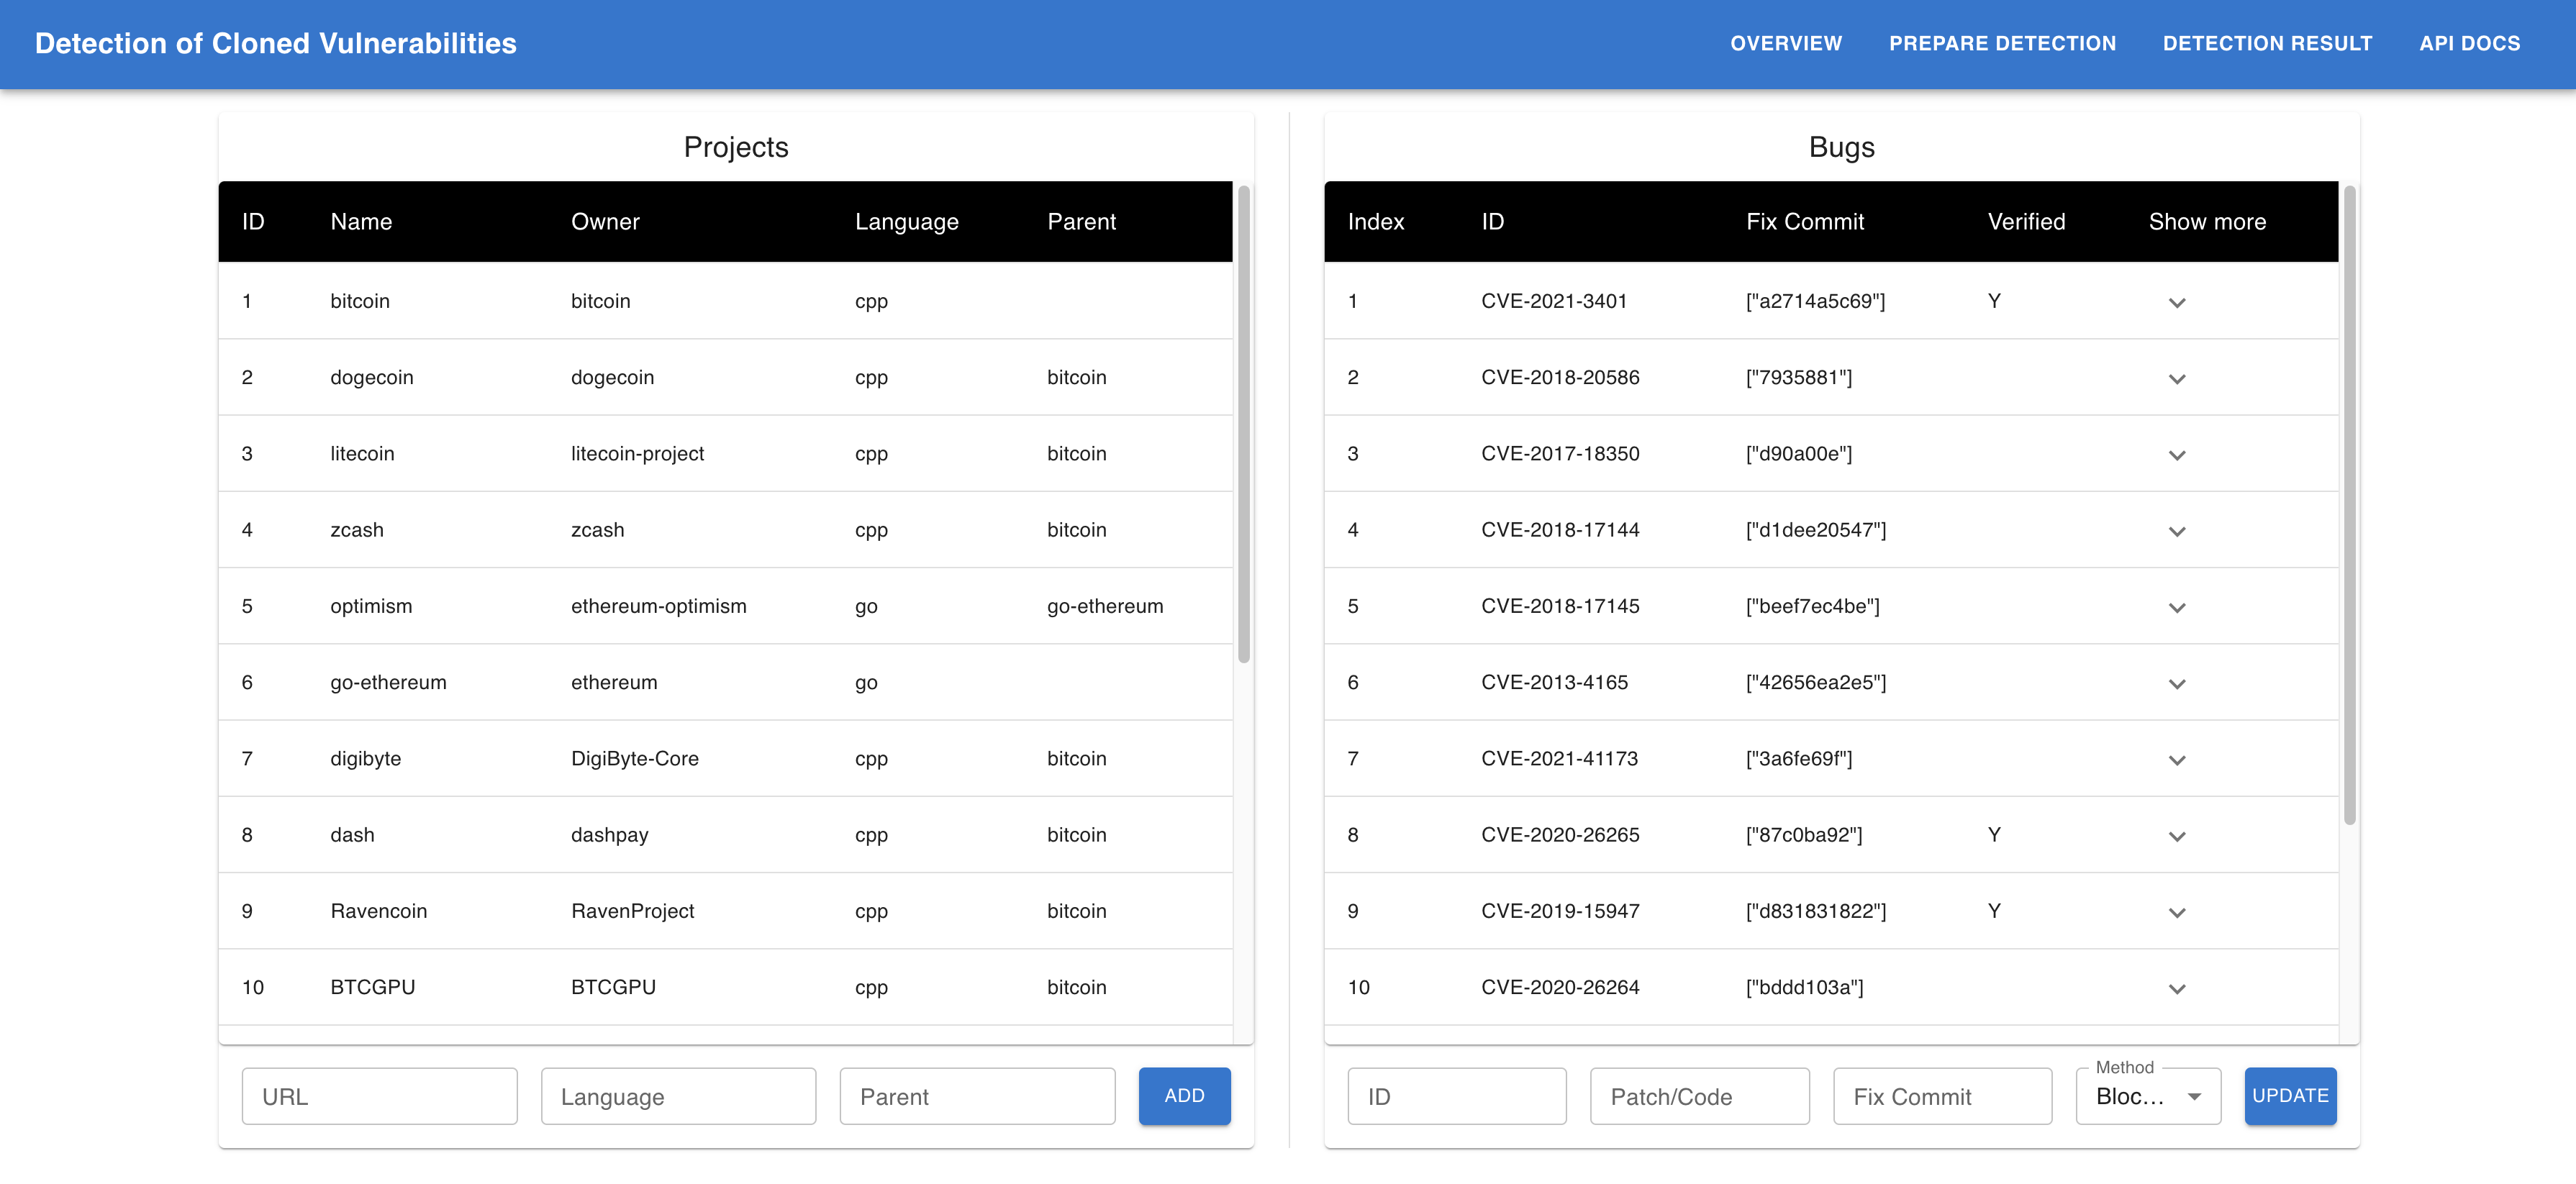
\includegraphics[width=1\textwidth]{obrazky-figures/cg_web_overview.png}
    \caption{Implemented overview web page.}
    \label{cg-impl-overview}
  \end{figure}

  \begin{figure}[h]
    \centering
    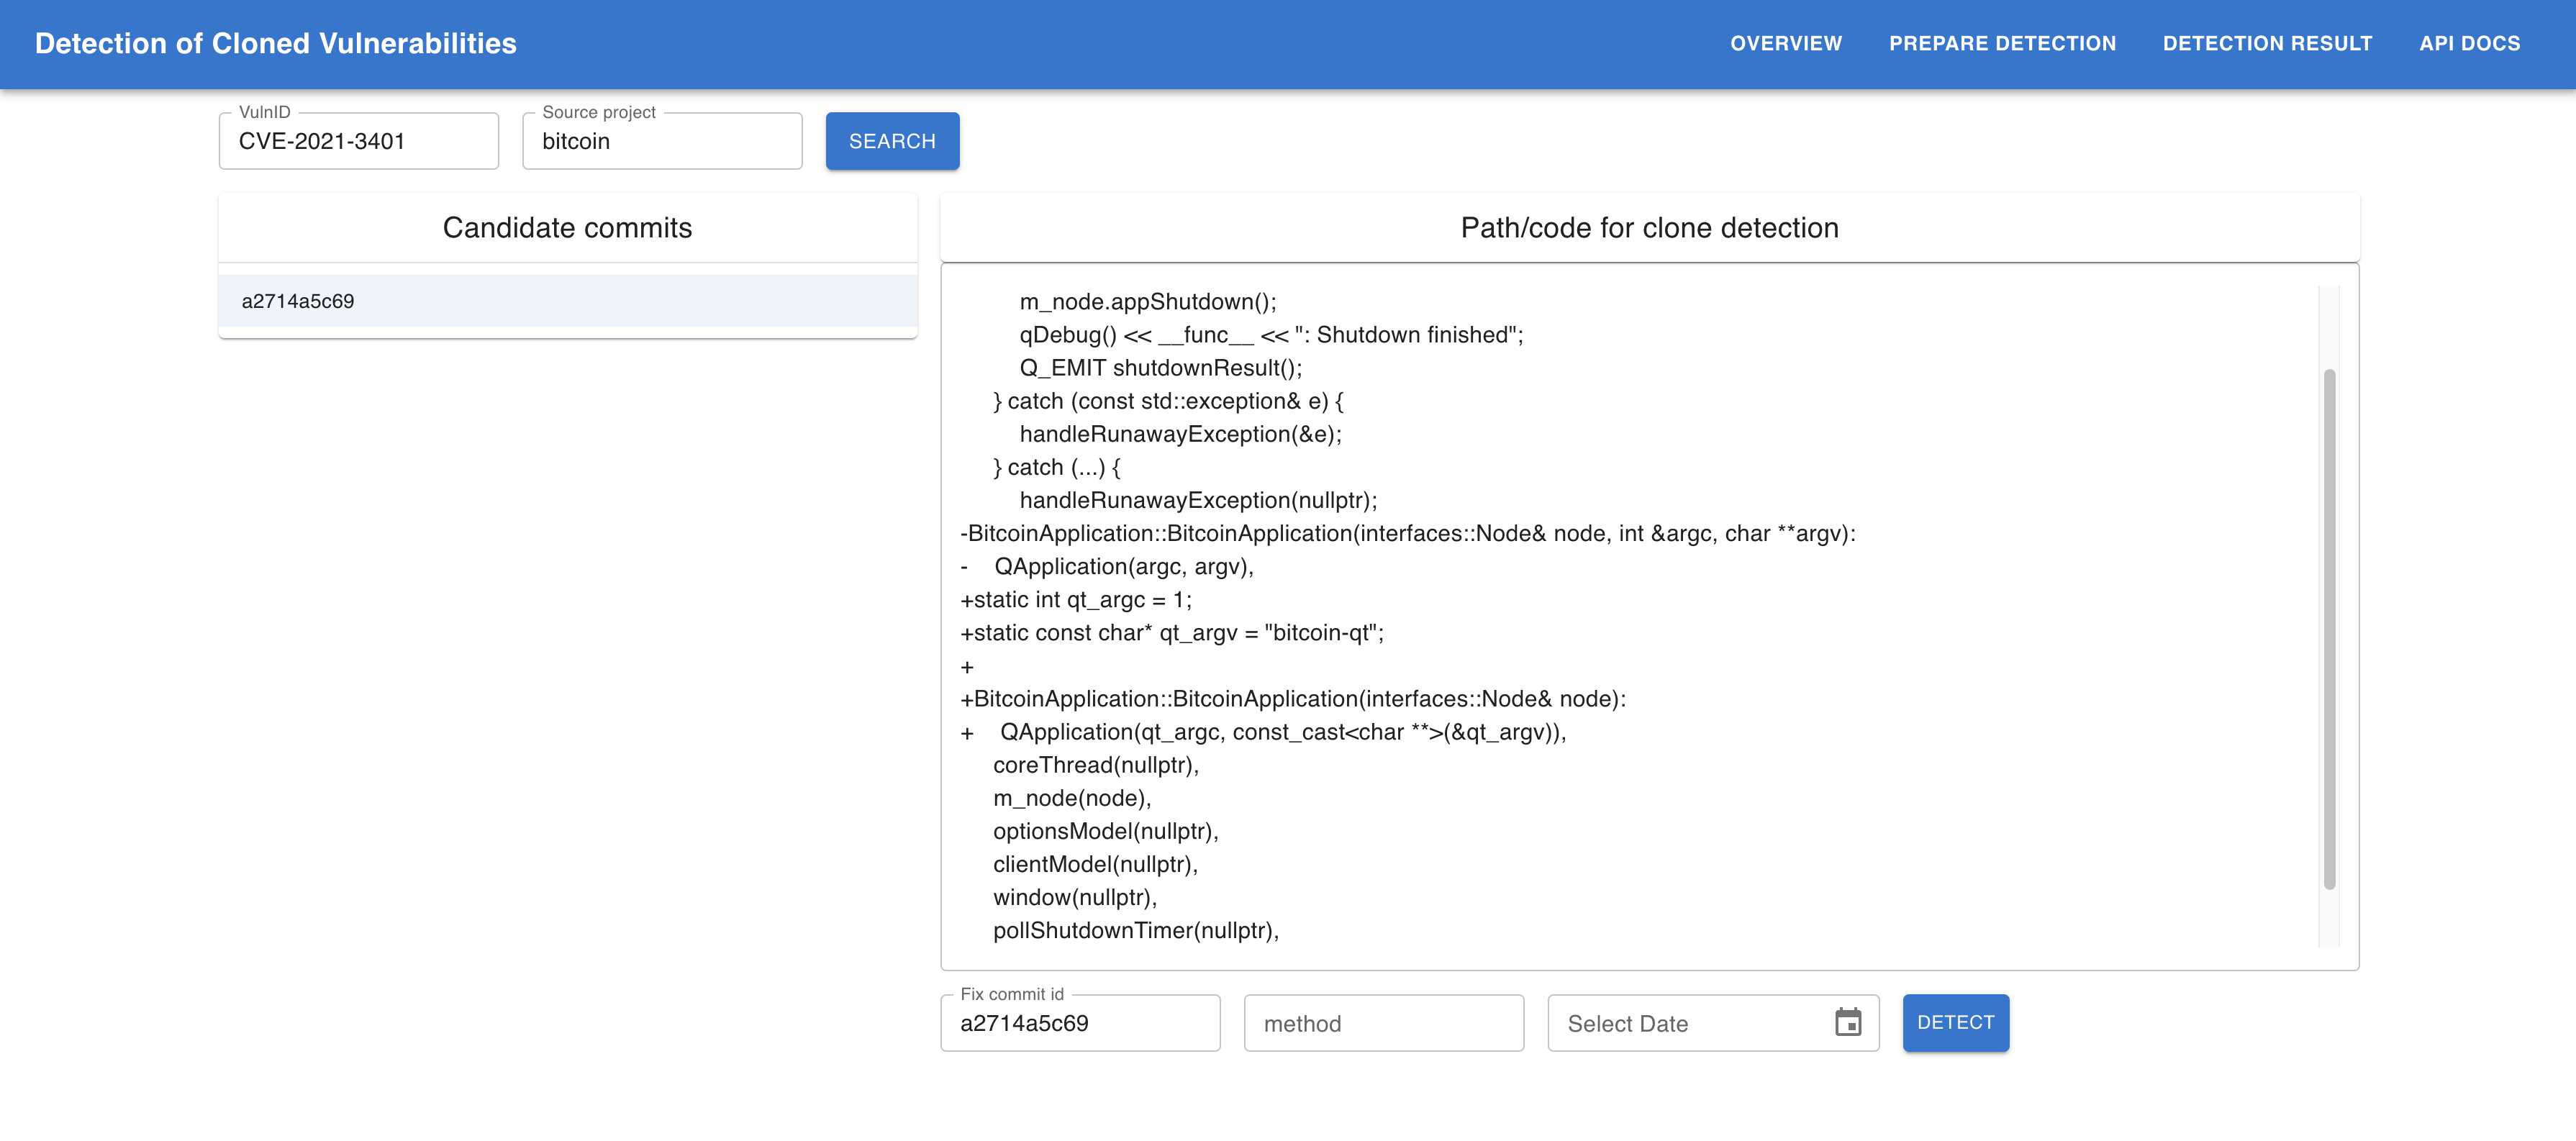
\includegraphics[width=1\textwidth]{obrazky-figures/cg_web_search.png}
    \caption{Implemented prepare detection web page.}
    \label{cg-impl-search}
  \end{figure}

  The preview of the third page is observable in Figure~\ref{cg-impl-results}. The page displays log and parsed results
  from detection method run-time. To fetch required data the web uses the API endpoint \texttt{/detection/results}. The purpose of this page is informational and does not affect the method.

  \begin{figure}[h]
    \centering
    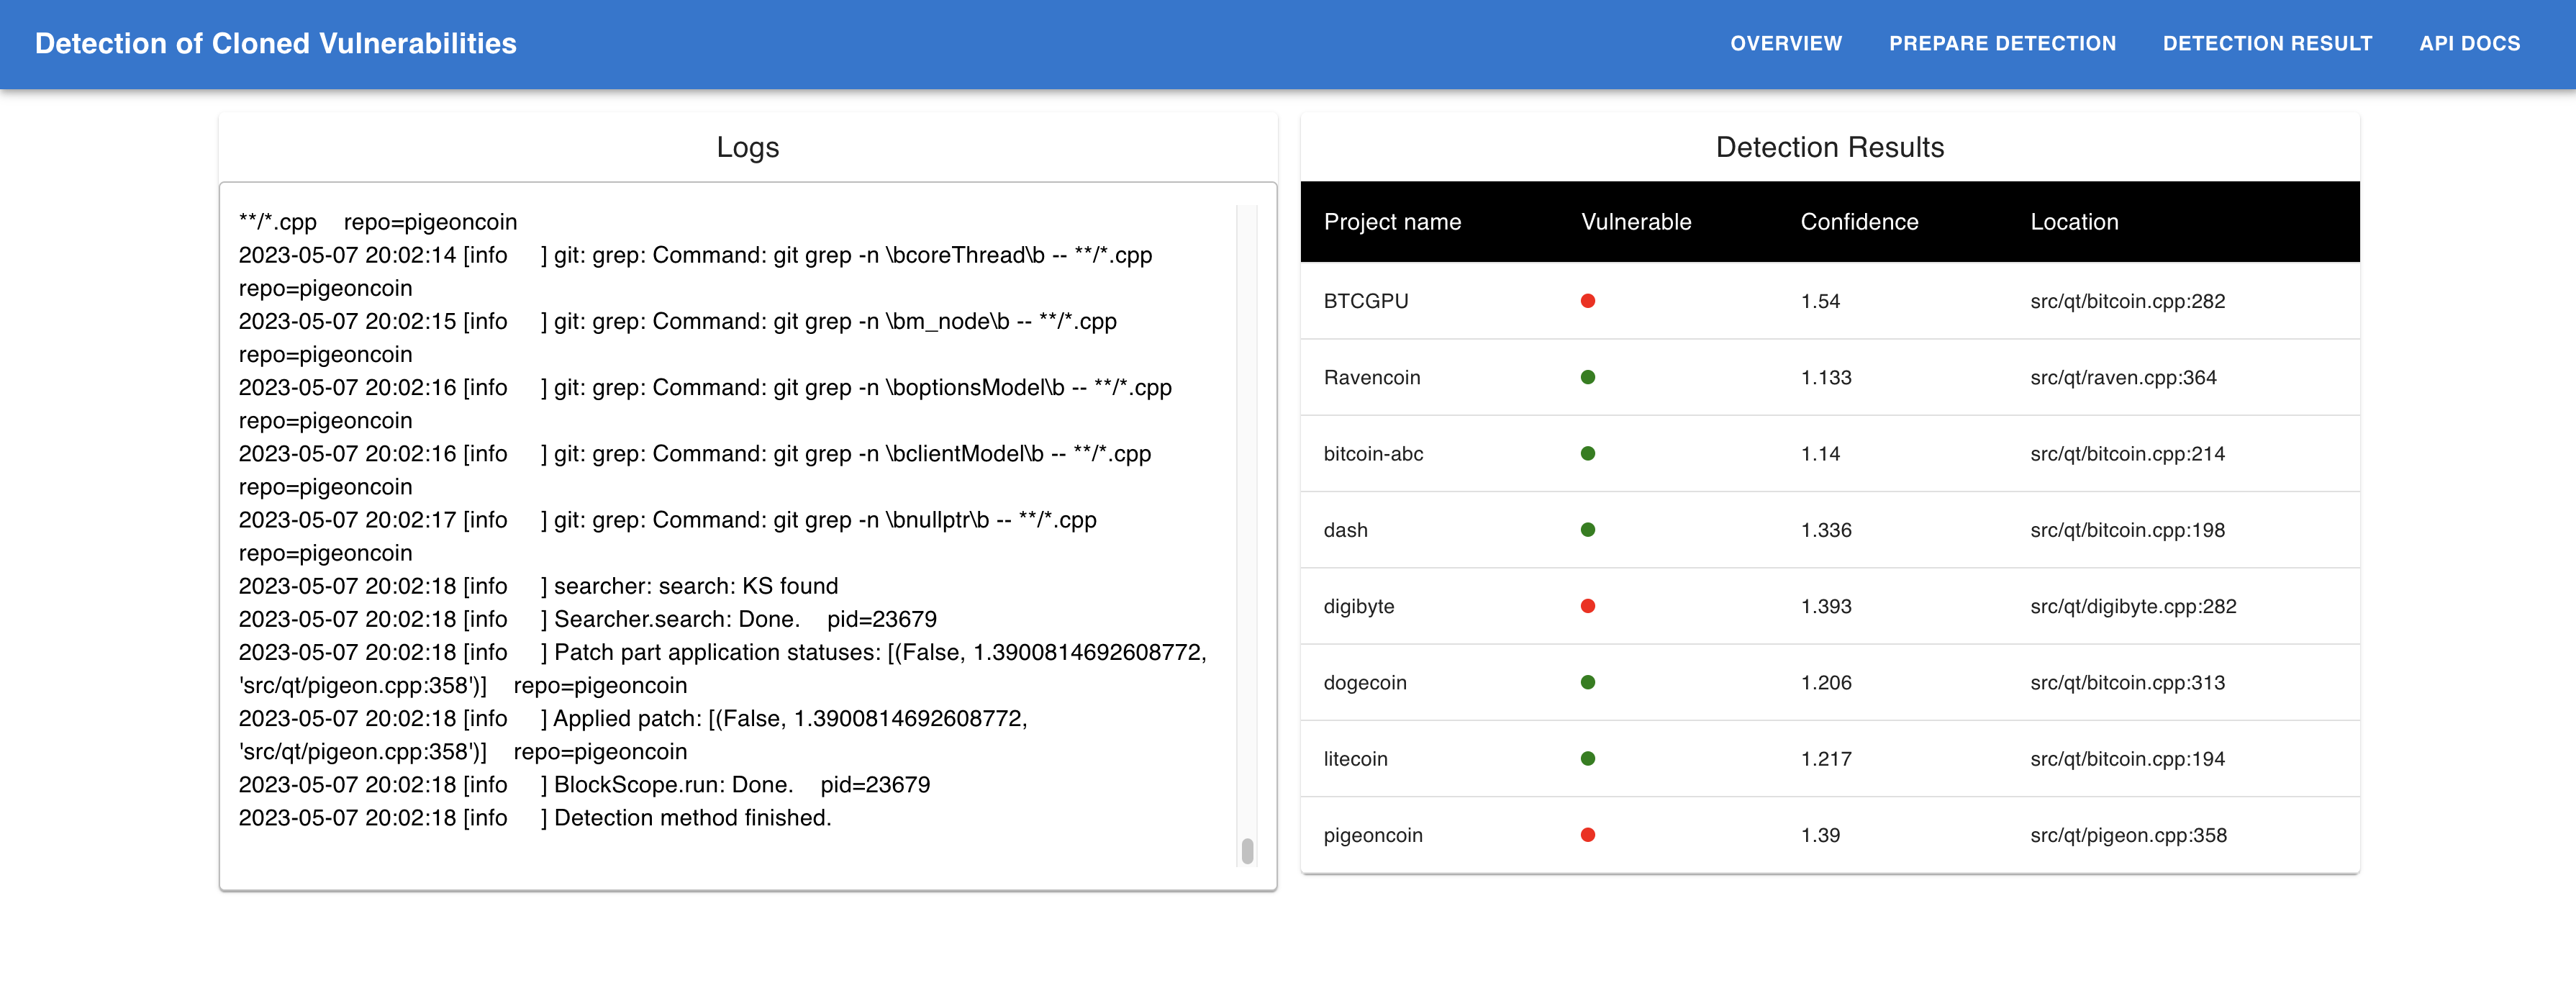
\includegraphics[width=1\textwidth]{obrazky-figures/cg_web_results.png}
    \caption{Implemented web page displaying detection logs and results of CVE-2021-3401.}
    \label{cg-impl-results}
  \end{figure}

  \subsection*{Command Line Interface}
  Additionally to the web, the tool provides also a command line interface (CLI), which benefits in terms of efficiency
  and lesser load on a~machine as it depends only on the database and Redis. Although, the output is not as clear as in the web interface
  and requires an experience with the command prompt.

  For implementation of the CLI a~Python library \texttt{click}\footnote{\href{https://click.palletsprojects.com/en/8.1.x/}
  {https://click.palletsprojects.com/en/8.1.x/}} was used. Its syntax reminds of the FastAPI as the commands and their arguments
  are defined using decorators. The decorators take care of parsing arguments, which makes the code shorter and more clear
  in comparison to other libraries, for example, Python built-in library \texttt{argparse}\footnote{\href{
  https://docs.python.org/3/library/argparse.html}{https://docs.python.org/3/library/argparse.html}}.

  The CLI implements the following commands, which are expecting the same values of arguments as in API:
  \begin{itemize}
      \item register and clone a~new project\\
      \texttt{\$ cli register <URL> <language> [\texttt{-}\texttt{-}parent <project>]}
      \item run targeted detection\\
      \texttt{\$ cli run <bug\_id> <project> <method> [\texttt{-}\texttt{-}date <date>]}
      \item run discovery scan with the option to set a~schedule for scans\\
      \texttt{\$ cli scan [schedule]}
      \item initialize the schema of the database \\
      \texttt{\$ cli db-init}
  \end{itemize}
